\documentclass[a4paper,11pt]{article}
\usepackage[utf8]{inputenc}
\usepackage{color,amsmath,xcolor,listings,graphicx}
\usepackage[francais]{babel}
\usepackage{hyperref}

%% paramétrage pour les zones de 'code'
\lstdefinelanguage{javascript}{
  keywords={typeof, new, true, false, catch, function, return, null, catch, switch, var, if, for, in, while, do, else, case, break},
  keywordstyle=\color{blue}\bfseries,
  ndkeywords={class, export, boolean, throw, implements, import, this},
  ndkeywordstyle=\color{darkgray}\bfseries,
  identifierstyle=\color{black},
  sensitive=false,
  comment=[l]{//},
  morecomment=[s]{/*}{*/},
  commentstyle=\color{purple}\ttfamily,
  stringstyle=\color{red}\ttfamily,
  morestring=[b]',
  morestring=[b]"
}

\lstset{
    language=javascript, commentstyle=\textit, frame=shadowbox,
    rulesepcolor=\color{gray}, basicstyle=\ttfamily\small, columns=flexible,
    tabsize=4, extendedchars=true, showspaces=false,
    showstringspaces=false, numbers=left, numberstyle=\tiny,
    breaklines=true, breakautoindent=true, captionpos=b, morecomment=[l]{//}
}


%% infos du document
\title{Filtres}
\author{Loïc Barbaresco, Rémi Barbaste, Robin Degironde, Émeric Tosi}
\date{\today}


\begin{document}

%% Afficher la page de garde : Titre + Auteur(s) + Date de dernière compilation
    \maketitle{}

    \clearpage

    \setcounter{tocdepth}{3} % définir la profondeur de l'Index
    \renewcommand{\contentsname}{Sommaire} % renommer l'Index en Sommaire
    \tableofcontents{} % afficher l'Index

    \clearpage


\section{Définition}
    \paragraph{}
Un filtre est un dispositif (actif ou passif) qui permet de réaliser une opération de traitement du signal.
En effet, il permet de transformer un signal reçu en entrée en un signal de sortie différent par le biais de circuits électroniques,
ces derniers servant à modifier le spectre de fréquence et/ou la phase du signal reçu.
    \paragraph{}
Les filtres permettent donc l’isolement, l’élimination ou la séparation de signaux.
Ce traitement peut par exemple consister à éliminer ou affaiblir des fréquences parasites (comme du bruit),
et/ou à isoler une information utile présente au sein d'une certaine bande passante d'un signal.
    \\
    \begin{figure}[h]
        \begin{center}
            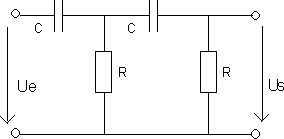
\includegraphics[scale=0.7]{images/filtres/filtre-passif.jpg}
        \end{center}
            \caption{ Un filtre passif }
            \label{Un exemple de filtre passif}
    \end{figure}
    \\
    \begin{figure}[h]
        \begin{center}
            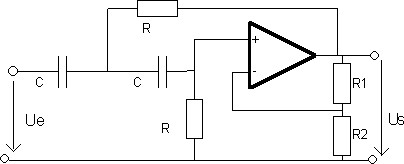
\includegraphics[scale=0.7]{images/filtres/filtre-actif.jpg}
        \end{center}
            \caption{ Un filtre actif }
            \label{Un exemple de filtre actif}
    \end{figure}

    \clearpage


\section{Différences entre filtre analogique et numérique}
    \paragraph{}
Parmi les différents filtres existants, on peut les classer selon deux catégories : analogiques ou numériques.
    \paragraph{}
Un filtre analogique permet de traiter de façon analogique un signal en retirant les signaux indésirables afin de ne conserver que le signal utile.
De ce fait, le signal qui le traverse est diffèrent en sortie que celui présent en entrée, cette modification est appliquée directement au signal.
    \paragraph{}
Un filtre numérique permet de traiter numériquement un signal.
Pour cela, le signal est numérisé sur le support en entrée, grâce par exemple à un convertisseur analogique-numérique (CAN) afin d’échantillonner ce signal.
On modifie, vérifie ou trie ensuite ces informations binaires constituant un flux de données.
On émet finalement un nouveau signal généré à partir de ce flux binaire de données sur le support en sortie grâce par exemple à un convertisseur numérique-analogique (CNA).

    \clearpage


\section{Différences entre filtre passif et actif}
    \paragraph{}
Les filtres passifs sont composés uniquement d’éléments passifs (c’est-à-dire des éléments résistifs, capacitifs et inductifs).
De ce fait, le gain d’un tel filtre ne peut excéder 1. Un tel type de filtre ne peut qu’atténuer une partie d’un signal,
il ne peut donc pas être utilisé dans le but d’amplifier un signal.
Les réalisations les plus simples sont réalisées à partir de circuits RC ou RL, cependant on peut trouver des associations diverses de composants (comme LC ou RLC),
mais ces circuits sont plus complexes.
    \paragraph{}
Les filtres actifs contiennent au moins un élément actif, comme un transistor ou un amplificateur opérationnel, qui va amplifier le signal.
Avec un tel filtre, il est possible d’avoir un gain supérieur à 1.
On peut les utiliser pour atténuer tout comme pour amplifier certaines fréquences d’un signal.
    \paragraph{}
Toutefois lors de l’utilisation des hautes fréquences, le problème qui se pose est que la notion de filtre ne signifie plus rien.
Tous les composants, y compris les lignes électromagnétiques, constituant le filtre possèdent une atténuation,
des capacités et des inductances qui influent sur le résultat du filtre.
La fonction d’amplificateur opérationnel n’existe pas non plus.

%    \clearpage


\section{Comparaison de filtres}

    \begin{tabular}{|c|c|c|c|c|c|}
        \hline
                        & Butterworth   & Tchebycheff   & Cauer     & Bessel    & Legendre  \\
        \hline
            Coupure     & +             & ++            & +++       & +         & +++       \\
        \hline
            Ondulation  & ++            & -             & -         & ++        & +++       \\
        \hline
            Distorsion  & ++            & +             & -         & +++       & ++        \\
        \hline
            Calculs     & ++            & +++           & +         & ++        & -         \\
        \hline
            Réalisation & +++           & ++            & +         & +++       & -         \\
        \hline
    \end{tabular}

    \subsection{Butterworth}
        \paragraph{}
Le filtre de Butterworth est un filtre polynômial qui possède un gain qui est constant dans la bande passante.
En effet, il possède une réponse qui est la plus plate possible, il n’y a pas d’ondulation.
Un tel filtre est le seul filtre linéaire qui a une forme générale qui est similaire quelque soit l’ordre.
De plus, la fréquence de coupure possède toujours un affaiblissement de -3dB.

    \subsection{Tchebyscheff}
        \paragraph{}
Le filtre de Tchebycheff est, tout comme le filtre de Butterworth, un filtre polynômial.
Il possède cependant une meilleure sélectivité que ce dernier, mais sa courbe de réponse en bande passante présente des ondulations (il y en a n dans la bande passante, n étant la valeur de l'ordre du filtre).
Sa coupure est un peu plus raide que pour un filtre de Butterworth.

    \subsection{Cauer}
        \paragraph{}
Le filtre de Cauer, également appelé filtre elliptique, possède une ondulation à la fois en bande passante et en bande atténuée.
La coupure est ici bien plus raide que les deux précédents filtres.
Les signaux subissent en revanche une déformation assez importante.

    \subsection{Bessel}
        \paragraph{}
Le filtre de Bessel, qui est également un filtre polynômial, offre un délai constant dans sa bande passante et une conservation de la phase des fréquences, la distorsion est donc minimale.
La coupure est moins raide que celle d’un filtre de Butterworth.

    \subsection{Legendre}
        \paragraph{}
Le filtre de Legendre, lui aussi polynômial, possède à la fois une atténuation monotone et une raideur maximale proche de la fréquence de coupure.
Il n’y a pas d’ondulation dans la bande passante.
On peut comparer la  raideur de coupure de ce filtre avec celle des autres filtres, on remarque qu’elle tend vers celle des filtres elliptiques.

    \clearpage{}

    \section{Notre outil logiciel de calcul}
        \paragraph{}
Afin de réaliser un programme de calcul des filtres passe-bas de Tchebyscheff,
nous avons choisi d’utiliser du JavaScript (pour la partie traitement) associé au couple HTML/CSS (pour la partie rendu et affichage).
Dans la partie JavaScript, nous calculons les valeurs des éléments localisés Lk, Ck et Rn à partir des caractéristiques du filtre.
Ces dernières, fournies par l'utilisateur, sont l’ordre, le taux d’ondulation maximal, la fréquence de coupure ainsi que l’impédance R1.
        \paragraph{}
A partir des valeurs saisies, nous calculons la pulsation, la valeur de beta et de gamma,
ensuite la valeur de R en appliquant la bonne formule selon si l’ordre est pair ou impair.
Puis nous déterminons les valeurs des Ak, Bk, Gk, L, C.
        \paragraph{}
Nous affichons les résultats sous la forme d’un tableau en indiquant l’ordre,
la valeur du condensateur C, celle de l’inductance L et celle de la résistance R.
    \\
    \begin{figure}[h]
        \begin{center}
            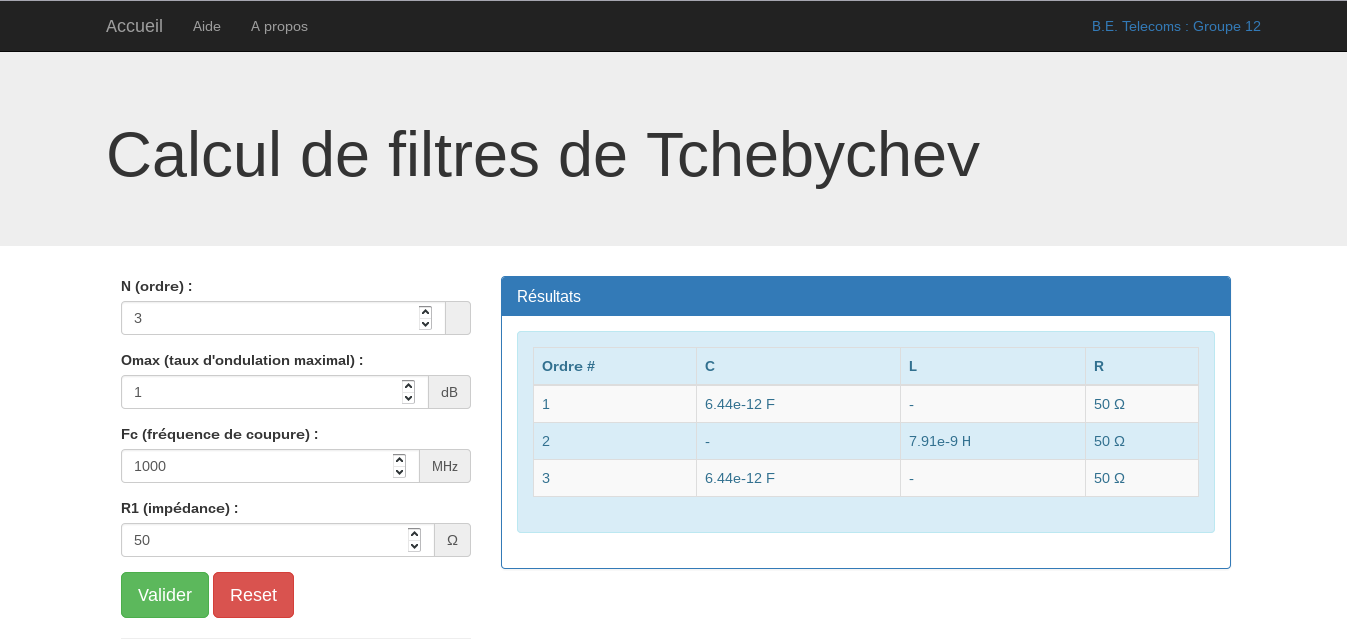
\includegraphics[scale=0.3]{images/filtres/screen-site.png}
        \end{center}
            \caption{ La page de calcul de notre outil }
            \label{La page de calcul de notre outil de calcul de filtres de Tchebyscheff}
    \end{figure}

    \clearpage


\section*{Annexes}
\addcontentsline{toc}{section}{Annexes}

    \subsection*{Code HTML}
\addcontentsline{toc}{subsection}{Code HTML}
\lstset{
    language=html, commentstyle=\textit, frame=shadowbox,
    rulesepcolor=\color{gray}, basicstyle=\ttfamily\small, columns=flexible,
    tabsize=4, extendedchars=true, showspaces=false,
    showstringspaces=false, numbers=left, numberstyle=\tiny,
    breaklines=true, breakautoindent=true, captionpos=b, morecomment=[l]{//}
}
        \lstinputlisting{../Filtres/sources/index.html}

    \clearpage

    \subsection*{Code JavaScript}
\addcontentsline{toc}{subsection}{Code JavaScript}
\lstset{
    language=javascript, commentstyle=\textit, frame=shadowbox,
    rulesepcolor=\color{gray}, basicstyle=\ttfamily\small, columns=flexible,
    tabsize=4, extendedchars=true, showspaces=false,
    showstringspaces=false, numbers=left, numberstyle=\tiny,
    breaklines=true, breakautoindent=true, captionpos=b, morecomment=[l]{//}
}

    \subsubsection*{Calculs}
\addcontentsline{toc}{subsubsection}{Calculs}

        \paragraph{calcul de la pulsation}
        \[ W_{c} = 2 * \pi * \mbox{ Fréquence de coupure}\]
        \begin{lstlisting}
            /* pulsation */

            Wc = 2 * Math.PI * freqCoup;

        \end{lstlisting}

        \paragraph{calcul de beta}
        \[ \mbox{Béta } \beta = \log( \frac{ \cosh( \frac{ \mbox{Ondulation} }{17,37} ) } { \sinh( \frac{ \mbox{Ondulation} }{17,37} ) } )\]
        \begin{lstlisting}
            /* beta */

            beta = Math.log( ( cosh( ondulation / 17.37 ) ) / ( sinh( ondulation / 17.37 ) ) );

        \end{lstlisting}

        \paragraph{calcul de gamma}
        \[ \mbox{Gamma } \gamma = \sinh( \frac{ \beta }{ 2 * \mbox{Ordre} } ) \]
        \begin{lstlisting}
            /* gamma */

            gamma = sinh( beta / ( 2 * ordre ) );

        \end{lstlisting}

    \clearpage

        \paragraph{calcul de R}
        Si l'ordre est pair \[ R_{n} = ( \tanh{ \frac{ \beta }{ 4 } } ) ^2 * \mbox{Impédance} \]
        Si l'ordre est impair \[ R_{n} = \mbox{Impédance} \]
        \begin{lstlisting}
            /* calcul de R */

            if ( ( ordre % 2 ) != 0 )
            {
                R = 1;
            }
            else
            {
                R = tanh( beta / 4 ) * tanh( beta / 4 );
            }

            /* calcul de Rn */

            Rn = R * impedance;

        \end{lstlisting}

        \paragraph{calcul de Ak}
        \[ A_{k} = \frac{\sin{2 * (k-1) * \pi}}{2 * \mbox{Ordre}} \]
        \[ k \mbox{ étant la position du composant} \]
        \begin{lstlisting}
            /* calcul des Ak */

            for( k = 1; k <= ordre; k++ )
            {
                Ak[k] = Math.sin( ( ( 2 * k-1 ) * Math.PI ) / ( 2 * ordre ) );
            }

        \end{lstlisting}

    \clearpage

        \paragraph{calcul de Bk}
        \[ B_{k} = \gamma ^2 + \sin( \frac{k * \pi}{\mbox{Ordre}} ) ^2 \]
        \[ k \mbox{ étant la position du composant} \]
        \begin{lstlisting}
            /* calcul des Bk */

            for( k = 1; k <= ordre; k++ )
            {
                Bk[k] = gamma * gamma + Math.sin( k * Math.PI / ordre ) * Math.sin( k * Math.PI / ordre );
            }

        \end{lstlisting}

        \paragraph{calcul de Gk}
        \[ G_1 = 2 * \frac{A_1}{\gamma} \]
        \[ G_{k} = \frac{(4 * A_{k-1} * A_{k})}{B_{k-1} * G_{k-1}} \]
        \[ k \mbox{ étant la position du composant} \]
        \begin{lstlisting}
            /* calcul des Gk */

            Gk[1] = 2 * Ak[1] / gamma;

            for( k = 2; k <= ordre ; k++ )
            {
                Gk[k] = ( 4 * Ak[k-1] * Ak[k] ) / ( Bk[k-1] * Gk[k-1] );
            }

        \end{lstlisting}

    \clearpage

        \paragraph{calcul de Lk }
        \[ L_{k} = \frac{G_{k} * \mbox{Impédance}}{W_{c}} \]
        \[ k \mbox{ étant la position du composant} \]
        \begin{lstlisting}
            /* calcul des L */

            for( k = 1; k <= ordre ; k++ )
            {
                l[k] = ( impedance * Gk[k] ) / Wc ;
            }

        \end{lstlisting}

        \paragraph{calcul de Ck }
        \[ C_{k} = \frac{G_{k}}{\mbox{Impédance} * W_{c}} \]
        \[ k \mbox{ étant la position du composant} \]
        \begin{lstlisting}
            /* calcul des C */

            for( k = 1; k <= ordre ; k++ )
            {
                c[k] = Gk[k] / ( ( impedance * Wc ) );
            }

        \end{lstlisting}

    \clearpage
    \subsubsection*{Code Complet}
\addcontentsline{toc}{subsubsection}{Code Complet}
        \lstinputlisting{../Filtres/sources/rsc/app.js}

    \clearpage

\end{document}
